%%=============================================================================
%% Conclusie
%%=============================================================================

\chapter{Conclusie}%
\label{ch:conclusie}

Deze bachelorproef richt zich op het adresseren van de inefficiënties en mogelijke fouten bij het handmatig beheren van IP-registraties binnen het netwerk van UGent. Dankzij de ontwikkeling van een nieuwe registratietool, bestaande uit de combinatie van Python-scripts, een gebruiksvriendelijke webinterface, en DDI-systeem EfficientIP, worden aanzienlijke verbeteringen gerealiseerd in termen van efficiëntie, tijdsbesparingen en het verminderen van fouten.

De registratietool maakt het mogelijk voor gebruikers om eenvoudig IP-registraties aan te vragen door middel van een intuïtieve interface, waarbij de complexiteit van het selecteren van de juiste subnetten wordt verminderd door gebruik te maken van keuzelijsten op basis van campus- en gebouwen en achterliggende codes. Dit leidt tot een vereenvoudigde aanpak en heeft het potentieel om menselijke fouten te verminderen. 

Daarnaast is er een afzonderlijke pagina gemaakt op de registratietool waarop de netwerkbeheerders de gemaakte registraties of wijzigingen kunnen nakijken, en goed- of afkeuren.

\section{Metingen}
Zoals te zien in figuur \ref{fig:tijdverbruik_metingen} blijkt dat het aanmaken, wijzigen en verwijderen van registraties aanzienlijke tijd in beslag neemt voor netwerkbeheerders. Dagelijks wordt er gemiddeld 17 minuten en 54 seconden besteed aan het exlusief uitvoeren van registratietaken, hierbij wordt geen rekening gehouden met variabelen zoals het aantal te verwerken registraties, de tijd die verloren gaat aan het verbinden met de server, het starten van de handmatige registratieprocessen of andere externe factoren. Deze bevindingen benadrukken de noodzaak om het beheer van IP-registraties te verbeteren en te automatiseren, wat een significante tijdsbesparing en efficiëntiewinst kan opleveren voor netwerkbeheerders.

\begin{figure}[H]
    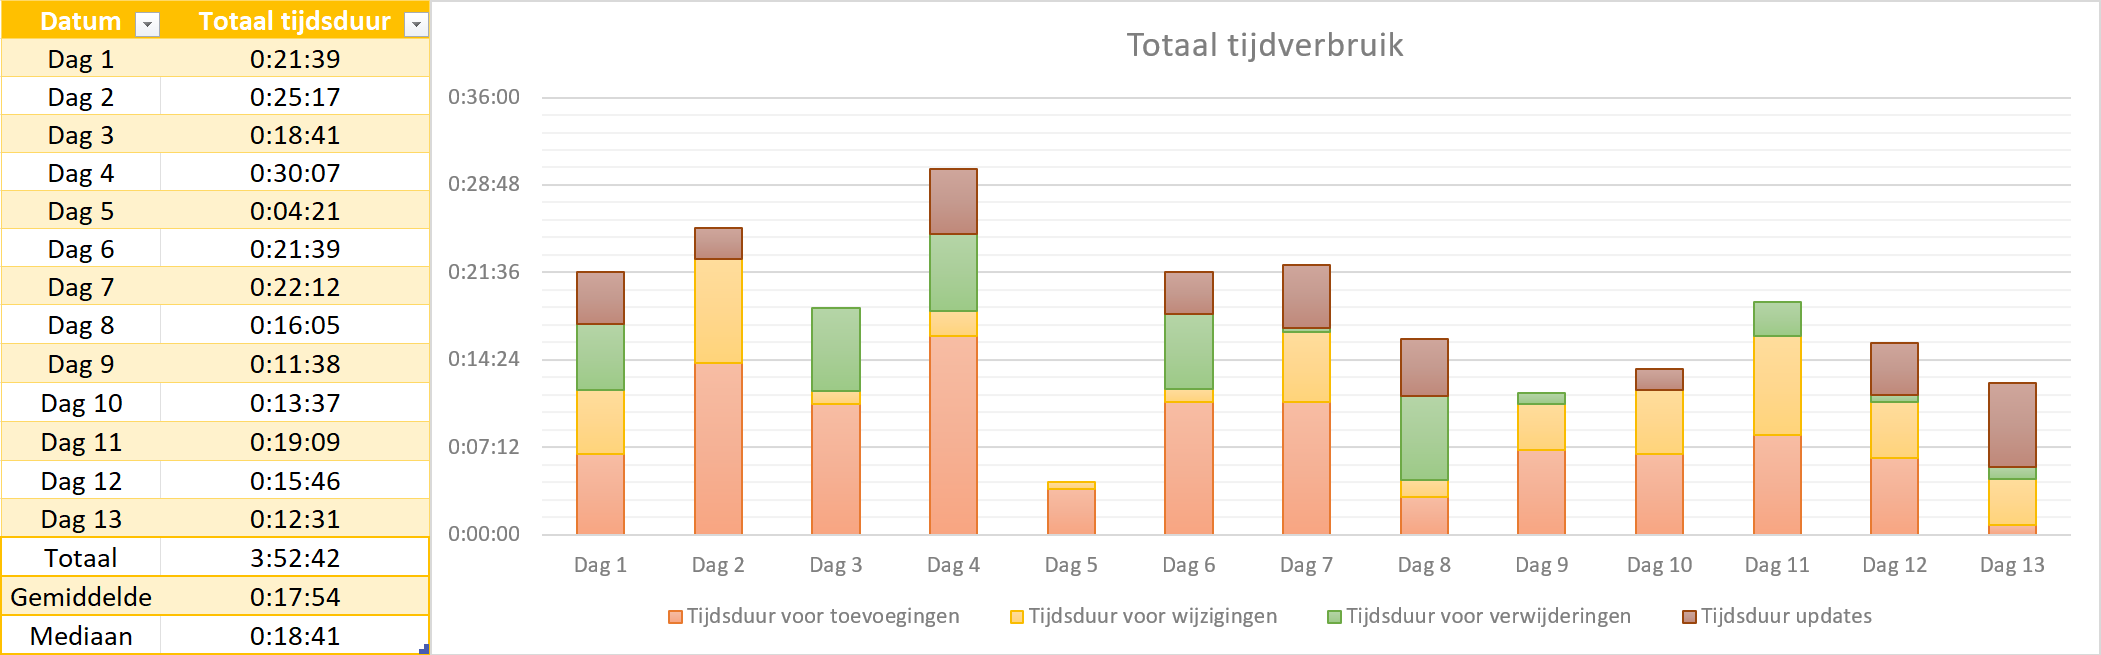
\includegraphics[width=16cm]{grafiek_totaal_tijdverbruik.png}
    \caption{Tabel en grafiek met totaal tijdverbruik tijdens metingen}
    \label{fig:tijdverbruik_metingen}
\end{figure}

\section{Verder onderzoek}
Deze registratietool geeft meerdere mogelijkheden voor verdere verbeteringen, zoals het implementeren van een API voor systeembeheerders en het mogelijk maken van bulkregistraties voor gebruikers, die toekomstig onderzoek rechtvaardigen.

In essentie levert dit onderzoek een waardevolle bijdrage aan het domein van netwerkbeheer door het ontwikkelen van een innovatieve aanpak voor het beheren en toewijzen van netwerkadressen. Deze aanpak biedt niet alleen tastbare voordelen voor de netwerkbeheerders van UGent, maar heeft ook het potentieel om als model te dienen voor vergelijkbare organisaties die worstelen met vergelijkbare uitdagingen in netwerkbeheer.

% TODO: Trek een duidelijke conclusie, in de vorm van een antwoord op de
% onderzoeksvra(a)g(en). Wat was jouw bijdrage aan het onderzoeksdomein en
% hoe biedt dit meerwaarde aan het vakgebied/doelgroep? 
% Reflecteer kritisch over het resultaat. In Engelse teksten wordt deze sectie
% ``Discussion'' genoemd. Had je deze uitkomst verwacht? Zijn er zaken die nog
% niet duidelijk zijn?
% Heeft het onderzoek geleid tot nieuwe vragen die uitnodigen tot verder 
%onderzoek?



